\section{Integráció}

\subsection{A generált kód felépítése}

Amennyiben compact code placement beállítással generáltuk le a fileokat, csupán 4 számunkra hasznos file keletkezik:

\begin{itemize}

    \item "subsystem neve".c
    \item "subsystem neve".h
    \item rtwtypes.h
    \item ert\_main.c

\end{itemize}

A továbbiakban feltételezzük, hogy a generált subsystem neve "Controller" volt, az egyszerűbb olvashatóságért.

\begin{figure}[!ht]
    \centering
    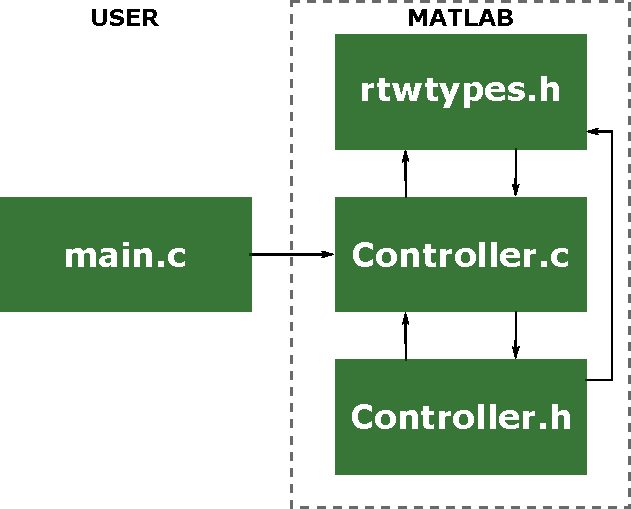
\includegraphics[width=0.6\linewidth]{img/rtw}
    \caption{A generált fileok kapcsolata}
    \label{fig:rtw}
\end{figure}

A \textbf{Controller.c} és \textbf{Controller.h} fileokban van definiálva a rendszer működése. A kódból hozzávetőlegesen kiolvasható a modell működése. A \textbf{rtwtypes.h} fileban kerülnek definiálásra a rendszer által használt típusok, az \textbf{ert\_main.c} pedig bemutatja a használatukat.

\subsection{Simulink modell kezelése C kódban}

A generált kód tökéletes megfelelője a Simulinkben futtatott modellnek. A generált fileok egy objektumot definiálnak, saját típusokkal és tagfüggvényekkel.

A rendszer inicializálását a Controller\_initialize() függvénnyel tehetjük meg. Ez a modell futásának elídításának felel meg, beállítja a 0 időpillanatot a rendszerben, a kimenetek felveszik az alapértelmezett értéküket.
A rendszerrel csupán a be és kimeneti interfészen keresztül kommunikálhatunk, valamint hatást gyakorolhatunk rá a \verb!Step! függvény meghívási idejének változtatásával (ezt nem részletezzük, és ne is nagyon erőltessük).
A bemeneti interfészt a Controller\_U struktúra implementálja, ennek a változónak a tagjai felelnek meg egy-egy bemeneti jelnek.\footnote{Többdimenziós jel esetén tömbként történik az átadás. 2 vagy több dimenzió esetén ne feledjük, hogy a MATLAB \textbf{oszlopfolytonosan} kezeli a tömböket.}

Miután beállítottuk a bemeneteket, a Controller\_step() függvény meghívásával \textbf{léptethetjük} a modellt. A lépés megegyezik a generált rendszer \textbf{1 mintavételi idejű} lépésével. A Step függvény lefutása közben frissülnek a rendszer belső állapotai, valamint Controller\_Y-ban a kimenetek. A kimenetet hasonlóléppen állítja elő a rendszer, Controller\_Y struktúrában tárolva.

A bemenetek megadása, léptetés, kimenet kiolvasása az az elemi lépéssorozat, melyet rendszeresen \textbf{időzítva} végrehajtunk. Ha a modellnek időtől függő belső állapotai is vannak\footnote{Ez minden esetben igaz, P szabályzónál bonyolultabb irányítás esetében}, \textbf{pontos időzítéssel} kell biztosítanunk a periodikus meghívást. Ha a rendszer túlnyomó része MATLAB-ban készült, ez csupán timer időzítővel is biztosítható, ám ha más feladatokat is el kell látnia a rendszernek, valószínűleg egy Hard Real-Time operációs rendszerre is szükségünk lesz.

\subsection{A FreeRTOS operációs rendszer}

A FreeRTOS egy szabadon felhasználható Real-Time operációs rendszer. Módosított GPL licence alatt fejlesztik, miszerint üzleti felhasználása esetén szerepelhet zárt forráskódú projektben, viszont a kernelt nyílt forráskóduvá kell tenni, és kérésre kiadni.\footnote{Létezik támogatott változata is, (...)}

A \verb!FreeRTOS! segítségével gyors és hatékony futást érhetünk el, és biztosíthatjuk a pontos időzítést, a többi adatgyűjtő taszk mellett is.

\subsection{Példarendszer integrációja periodikus meghívással}

A következő példa szemlélteti a generált kód integrálásának módját egy egyszerű kormányvezérlő alkalmazással.